\documentclass[conference, onecolumn]{IEEEtran}
\usepackage[utf8]{inputenc}
\usepackage{graphicx}
\usepackage{booktabs}
\usepackage{listings} % code snippet
\usepackage{hyperref}
\usepackage{amsmath}

\begin{document}

\title{Can an LLM Judge Bug Report Reproducibility? An Agreement Study on Original and AI-Improved Mojira Reports}
\author{\IEEEauthorblockN{Author 1, Author 2, ... }
\IEEEauthorblockA{FPT University, Vietnam}}

\maketitle

\begin{abstract}

\label{sec:abstract}
Reproducing a reported bug is often the slowest step in triage, and judging
whether a bug report contains enough information to be reproduced is a manual,
time-consuming task performed by developers. Whether a large language model
(LLM) can perform this judgment reliably enough to assist that process is
untested: prior work uses LLMs to generate or improve bug reports, but rarely
validates them as reproducibility \emph{assessors} against human judgment. We
evaluate GPT-4o mini as an automated reproducibility evaluator on the ImproBR
replication package, which provides two forms of the same 139 Mojira Minecraft
bug reports: the original (\emph{Raw}) reports, and \emph{Improved} versions in
which an LLM pipeline has rewritten each report to be more complete. Each form
was independently annotated by two human reviewers along three structured
dimensions (Steps to Reproduce, Observed Behavior, Expected Behavior). Treating
the two forms as co-equal conditions, we convert both the human annotations and
the LLM output into a common 1--5 ordinal reproducibility score with a single
deterministic scoring function, and measure agreement with Cohen's kappa
against a pre-registered threshold of $\kappa \geq 0.70$.

On the Raw reports the model reaches $\kappa = 0.578$ (95\% bootstrap CI
$[0.471,\,0.684]$; accuracy $71.9\%$), a moderate but sub-threshold level of
agreement, close to the $\kappa_{\text{control}} = 0.674$ between the two human
annotators on the same reports. On the Improved reports, agreement falls to
$\kappa = 0.335$ (CI $[0.226,\,0.441]$; accuracy $62.6\%$), only fair and well
below the human ceiling on those reports ($\kappa_{\text{control}} = 0.556$).
The drop is driven by a significant optimistic bias that appears only on the
Improved form: a Wilcoxon signed-rank test is non-significant on Raw
($p = 0.452$) but strongly significant on Improved ($p < 10^{-6}$), where the
model rates 111 of 139 reports as reproducible (score $\geq 4$) against the
humans' 94, scoring higher than the annotator in 47 cases and lower in only 5.
Across both forms, agreement is highest on the structurally checkable Steps to
Reproduce dimension (Raw $\kappa = 0.693$, Improved $\kappa = 0.654$) and
collapses on Observed Behavior (Raw $\kappa = 0.289$, Improved $\kappa =
0.130$). A coarse binarized check (score $\geq 4$ as reproducible) remains high
on both forms ($87.1\%$ and $86.3\%$ accuracy). GPT-4o mini does not meet the
pre-registered bar on either form, and its reliability degrades precisely on
the AI-polished reports whose fluent surface it appears to over-trust ---
evidence that an LLM evaluator should be validated on the kind of text it will
actually score, and is best used as a human-supervised coarse pre-filter rather
than an autonomous evaluator.

\end{abstract}

\begin{IEEEkeywords}
large language models, bug reports, reproducibility, inter-rater agreement, empirical software engineering
\end{IEEEkeywords}
% Keywords: 4-6 từ, chữ thường, phân tách bằng dau phẩy
% Chuẩn hoa tên: dùng IEEE Thesaurus tại thesaurus.ieee.org
% Ví dụ: "large language models" (không viết "LLMs"), "software testing" (không "SW testing")

\section{Introduction}
\label{sec:intro}

Bug reports are critical input to the software development process. However, without the ability to reproduce a bug, developers cannot diagnose or fix it. Recent work shows that fewer than 8\% of bug reports on platforms like Jira meet the criteria for first-time reproducibility, creating a significant bottleneck in software maintenance. For large projects managing tens of thousands of reports monthly (such as TensorFlow or Django), automating the reproducibility evaluation step offers clear practical value.

Large language models (LLMs) like GPT-4o have shown promise in various software engineering tasks, including bug report analysis and improvement. Yet a critical gap remains: no prior work has measured whether an LLM can evaluate bug report reproducibility with sufficient agreement to developer judgment. Existing studies either use LLMs to generate or improve bug reports, or measure agreement between human raters alone---not between LLM evaluators and developer assessment.

This work addresses that gap by investigating whether an LLM-based reproducibility evaluator can achieve substantial agreement (Cohen's $\kappa \geq 0.70$) with manual human review. We use the ImproBR replication package~\cite{akyol2026improbr}, which is uniquely suited to the question because it contains two forms of the same 139 Mojira Minecraft bug reports: the original \emph{Raw} reports as submitted, and \emph{Improved} versions in which an LLM pipeline has rewritten each report to be more complete. Both forms were independently annotated by two human reviewers using the same rubric.

We treat the two forms as \emph{co-equal conditions} and run the identical evaluation on each. This lets us ask not only whether GPT-4o mini agrees with human reproducibility judgment on ordinary reports, but also whether that agreement holds up on reports that another LLM has already polished. The two conditions are complementary: the Raw condition tests the model on the messy text a triage system actually receives, while the Improved condition tests whether the model can still track human judgment when the surface text has been made fluent and complete-looking by AI. A large gap between the two would be a warning that an LLM evaluator can be misled by fluent presentation rather than genuine reproducibility.

The contribution is three-fold: we establish a reusable measurement protocol for LLM-as-evaluator agreement on bug report quality; we provide an empirical baseline for whether LLMs can reliably assist in bug triage on both original and AI-improved reports; and we show that the two answers differ, which has direct implications for anyone considering an LLM evaluator in a pipeline that already contains LLM-generated text.

\section{Related Work}
\label{sec:related}

Our study sits at the intersection of three lines of research: (i) empirical
work characterizing what makes bug reports useful, (ii) techniques that assess
and improve the \emph{steps to reproduce} (S2R) that determine whether a report
is reproducible, and (iii) the emerging use of large language models (LLMs) for
bug report analysis and as automated evaluators. We review each theme and then
position our contribution.

\subsection{Bug Report Quality and Information Completeness}
\label{sec:related:quality}

A long line of empirical research establishes that bug reports vary widely in
quality and that this variation directly affects triage and resolution effort.
Survey evidence from developers of large open-source projects shows a systematic
mismatch between the information developers most need---steps to reproduce,
stack traces, and test cases---and the information reporters typically
provide~\cite{zimmermann2010good}. Complementary quantitative studies model
report quality from surface and textual features and confirm that such features
predict how quickly a report is acted upon, framing quality assessment as a
largely automatable task~\cite{hooimeijer2007modeling}. Broader content analyses
across multiple projects further quantify how often key fields are missing and
trace the downstream consequences of incomplete reports for developers who must
recover the missing context~\cite{davies2014whats}. Collectively, this theme
motivates \emph{reproducibility} as the quality dimension of greatest practical
value, yet it treats quality mostly through proxy features rather than by
judging whether a report is actually reproducible.

\subsection{Reproducibility and the Quality of Steps to Reproduce}
\label{sec:related:s2r}

A second theme targets the S2R directly, since incomplete or ambiguous steps are
the dominant obstacle to reproducing a failure. Early tool support augmented the
reporting process itself, guiding Android reporters to produce more complete,
reproducible steps at submission time~\cite{moran2015autocompleting}. Later work
shifted toward automatically \emph{assessing} S2R quality: Euler identifies the
reported steps and flags missing or low-quality ones to give reporters
actionable feedback~\cite{chaparro2019assessing}, and more recent approaches
combine language understanding with app UI models so that natural-language steps
are grounded in concrete interface interactions~\cite{mahmud2025combining}.
Closest to our setting, ImproBR uses an LLM pipeline to detect and repair
missing or ambiguous S2R, observed behavior, and expected behavior on the Mojira
issue tracker, substantially raising the share of executable steps and fully
reproducible reports~\cite{akyol2026improbr}. A common thread, however, is that
these S2R techniques are built for GUI/mobile applications and rely on program
or dynamic analysis of a runnable app to establish the language-to-program
mapping---an assumption that does not transfer to a game issue tracker such as
Minecraft/Mojira, and none of them frames reproducibility assessment as a
measured agreement task against human judgment.

\subsection{Large Language Models for Bug Report Analysis and Evaluation}
\label{sec:related:llm}

The third theme concerns LLMs applied to software engineering and, increasingly,
as evaluators. Systematic reviews document the rapid adoption of LLMs across SE
tasks and note that data quality and rigorous evaluation---not merely model or
dataset scale---determine reliability~\cite{hou2024llm4se}. In parallel, the
``LLM-as-judge'' paradigm studies when a model's assessments can substitute for
human evaluation, together with the meta-evaluation methods and limitations that
govern their trustworthiness~\cite{li2024judges}. This literature makes clear
that an LLM used as an assessor must itself be validated against human
annotators using an explicit reliability metric, rather than assumed correct.

\subsection{Positioning of Our Work}
\label{sec:related:positioning}

Prior work either (i) characterizes bug report quality through proxy features
without judging actual reproducibility, (ii) assesses S2R quality for GUI/mobile
apps using program or dynamic analysis that is infeasible for the
Minecraft/Mojira domain, or (iii) applies LLMs to \emph{generate}, \emph{improve},
or \emph{classify} reports---including ImproBR on the same Mojira
data~\cite{akyol2026improbr}---without validating the LLM as a reproducibility
\emph{assessor}. Our study addresses this gap: we use an LLM to automatically
assess bug report reproducibility on Mojira and evaluate it directly against
human expert annotation, treating the LLM-as-judge concern
seriously~\cite{li2024judges} by reporting Cohen's Kappa against a pre-registered
threshold of $\kappa \geq 0.70$. Uniquely, we run this evaluation on \emph{both}
the original reports and the LLM-improved versions that ImproBR produces from
them~\cite{akyol2026improbr}, treating the two as co-equal conditions, which lets
us measure whether an LLM evaluator's agreement with humans holds up on text that
another LLM has rewritten. To our knowledge, this is the first study to benchmark
automated reproducibility assessment as a human-agreement task on this domain,
and the first to quantify how that agreement changes on AI-improved reports.

\section{Methodology}
\label{sec:method}

% ==================== LR START ====================

\subsection{Dataset}
\label{subsec:dataset}

In this study, we used the \texttt{RQ1} subset of the
\textit{ImproBR Replication Package}, which is publicly available on
Figshare~\cite{improbr2026dataset}. It contains 139 real-world bug
reports collected from Mojira, the official issue tracker for
Minecraft. We selected \texttt{RQ1} because it provides the report
content and manual labels required to evaluate the executability of
\textit{Steps to Reproduce} (S2R).

Each issue has two corresponding versions. The \textit{Raw} version
contains the original report submitted to Mojira before being processed
by ImproBR. The \textit{Improved} version is the corresponding output
of the ImproBR pipeline. In the Improved report, components such as S2R
may be added, clarified, or reorganized. The two versions were paired
using \texttt{issue\_key}, enabling a paired comparison of the same
issue under the Raw and Improved conditions.

Ground-truth labels were obtained from the manual evaluations included
in the replication package~\cite{improbr2026dataset}. Two independent
human annotators evaluated both report versions. Because our study
focuses on automatically assessing S2R executability, we used only the
S2R label. This label has two possible values:
\texttt{Executable} and \texttt{Non-Executable}. A report is labeled
\texttt{Executable} when its reproduction steps are sufficiently clear
for an evaluator to follow. A report is labeled
\texttt{Non-Executable} when missing, incorrect, or ambiguous
information prevents the evaluator from following the steps without
making additional assumptions.

The Raw condition contains 40 \emph{Executable} reports (28.8\%) and
99 \emph{Non-Executable} reports (71.2\%). The Improved condition
contains 94 \emph{Executable} reports (67.6\%) and 45
\emph{Non-Executable} reports (32.4\%). These ground-truth labels serve
as the reference for evaluating model predictions. Each prediction is
matched to its corresponding label using \texttt{issue\_key} and the
report condition (Raw or Improved).

The 139 issues were divided into three subsets:
\textit{Pilot}, \textit{Development}, and \textit{Holdout}. First,
26 issues were assigned to Pilot for checking the execution pipeline,
output schema, and prompt design. After excluding the Pilot issues, the
remaining 113 issues were divided into 75 Development issues and 38
Holdout issues. We used \texttt{seed}=210 to make this split
reproducible.

The Development set was used to refine the Full configuration and
conduct error analysis; its results were treated as calibration
evidence rather than a final independent performance estimate. The
Holdout set was reserved for the final evaluation. Splitting was
performed at the \texttt{issue\_key} level, so the Raw and Improved
versions of each issue were always assigned to the same subset. This
prevents pair-level leakage between the Development and Holdout sets.


\subsection{Experimental Setup and Pipeline}
\label{subsec:pipeline}

The experimental pipeline was implemented in Python and accessed the
OpenAI Chat Completions API through the \texttt{openai} SDK. We used
\texttt{gpt-4o-mini-2024-07-18} with
\texttt{temperature}=0 and \texttt{seed}=210. JSON mode was enabled
using \path|response_format={"type":"json_object"}|. The
\texttt{max\_tokens} parameter was not explicitly specified. Fixing
the model version and generation parameters reduces unnecessary output
variation and supports reproducibility, although it does not guarantee
identical responses across repeated executions.

We used separate prompt templates for the Raw and Improved conditions.
Each template consists of System and User sections. The System section
defines the model's role, evaluation rubric, allowed label values, and
JSON output requirement. The User section supplies the
\texttt{issue\_key}, report content, and required JSON schema. The Raw
prompt instructs the model to evaluate only the Raw report. The
Improved prompt specifies the Improved report as the evaluation target
and includes its paired Raw report only as context for preserving the
original issue intent. Owing to the page limit, the complete prompt
texts are provided in the replication package.

During the Pilot phase, we used the Raw V10 and Improved V18 prompts,
both based on the rubric defined in
\path{evaluation_metrics.yaml}. For the Full phase, Raw V11 and
Improved V20 were refined on the Development set. Improved V20 combines
the V19 prompt with Rules V20. The resulting Full configurations were
then evaluated on the same 26 Pilot issues during Pilot Validation.

Post-processing rules were defined according to the evaluation rubric.
Pilot-specific rules were refined during the Pilot phase, whereas rules
for the Full configuration were calibrated only on the Development
set. During inference, these rules inspect the target report and, where
applicable in the Improved condition, its paired Raw context.
Ground Truth and prior predictions are not available to the rules.
Holdout labels and mismatches were not used for prompt refinement or
rule calibration.

After Pilot Validation, we froze the model version, prompts,
experimental script, post-processing rules, and metric logic. We
recorded SHA-256 hashes of the frozen files to verify their integrity
before the Holdout evaluation. The frozen configuration was then
evaluated once on the 38 Holdout issues for each condition. Holdout
results were not used for further tuning.

For each issue, the pipeline reads the common fields
\emph{Issue Key}, \emph{Summary}, \emph{Type},
\emph{Affects Version/s}, \emph{Labels}, \emph{Category}, and
\emph{Description}. Improved reports additionally include
\emph{Steps to Reproduce}, \emph{Observed Behavior},
\emph{Expected Behavior}, and \emph{Environment}. Ground Truth,
annotator labels, prior predictions, and potentially biasing
administrative fields---including \emph{Confirmation Status},
\emph{Resolution}, \emph{Fix Version/s}, \emph{Votes}, and
\emph{Watch Count}---are excluded from the prompt.

For the Raw condition, the Raw report is inserted into the
corresponding Raw prompt. For the Improved condition, the Improved
report is the evaluation target, while its paired Raw report is
included only as original-intent context. Each issue in each condition
is processed through one application-level API request. Ground Truth
is not included in the request and is introduced only during metric
computation.

The model is required to return a structured JSON object containing
the \texttt{issue\_key}; the S2R label, reproducibility, validity,
failure type, and rationale; auxiliary assessments of Expected and
Observed Behavior; and an overall rationale. The
\path{run_experiment.py} script reads the CSV input, identifies the
\texttt{issue\_key}, constructs the prompt, calls the API, parses the
response, applies the post-processing rules, and stores the result.

After receiving a response, the pipeline checks whether it is valid
JSON, verifies that all required fields are present, normalizes allowed
label values, and checks logical consistency among the fields. If an
API error, empty response, malformed JSON, or missing required field
occurs, the script records the case with status \texttt{error} and
continues with the next issue. The experiment script does not implement
an additional retry loop.

Structured predictions are stored in
\path{*_llm_output_*.csv}, while API status, model and prompt versions,
seed, \texttt{system\_fingerprint}, token usage, and cost are stored in
\path{*_api_log_*.csv}. Predictions are then matched with Ground Truth
using both \texttt{issue\_key} and the corresponding condition
(Raw or Improved). The merged data are passed to
\path{compute_metric.py}, which computes Accuracy, Cohen's Kappa, the
confusion matrix, and the list of mismatched cases. The source code,
prompts, data splits, and raw experimental outputs required for
replication are available at
\url{https://github.com/LamSongToan/SWT301_SE1925_G6}.

% ===================== LR END =====================
% ===================== MS START ===================

% MS writes Metrics and Statistical Analysis Plan below.

\section{Results}

\subsection{Experimental Overview}

The full experiment was conducted on 139 bug reports collected from the
Minecraft issue tracking dataset. Each report was independently annotated
using the proposed quality assessment framework and assigned a quality score
ranging from 1 to 5.

Two prompting strategies were evaluated:

\begin{itemize}
    \item Raw Prompt
    \item Improved Prompt
\end{itemize}

The outputs generated by the Large Language Model (LLM) were compared
against the human-annotated ground truth. Performance was evaluated using
Accuracy, Macro Precision, Macro Recall, Macro F1-score, and Cohen's Kappa.
In addition, confusion matrices and score distributions were analyzed to
provide further insights into the agreement patterns between the LLM and
human annotations.

\subsection{Raw Prompt Results}

Table~\ref{tab:raw_results} summarizes the performance obtained using the
Raw Prompt configuration.

\begin{table}[!t]
\centering
\caption{Performance Metrics for Raw Prompt}
\label{tab:raw_results}
\begin{tabular}{lc}
\toprule
Metric & Value \\
\midrule
Accuracy & 69.18\% \\
Precision (Macro) & 56.07\% \\
Recall (Macro) & 55.01\% \\
F1-score (Macro) & 53.22\% \\
Cohen's Kappa & 0.5776 \\
\bottomrule
\end{tabular}
\end{table}

The Raw Prompt configuration achieved moderate performance across all
evaluation metrics. The overall Accuracy reached 69.18\%, while the Macro
F1-score was 53.22\%, indicating that the model experienced difficulty in
maintaining consistent prediction quality across all score categories.

\begin{figure}[!t]
\centering
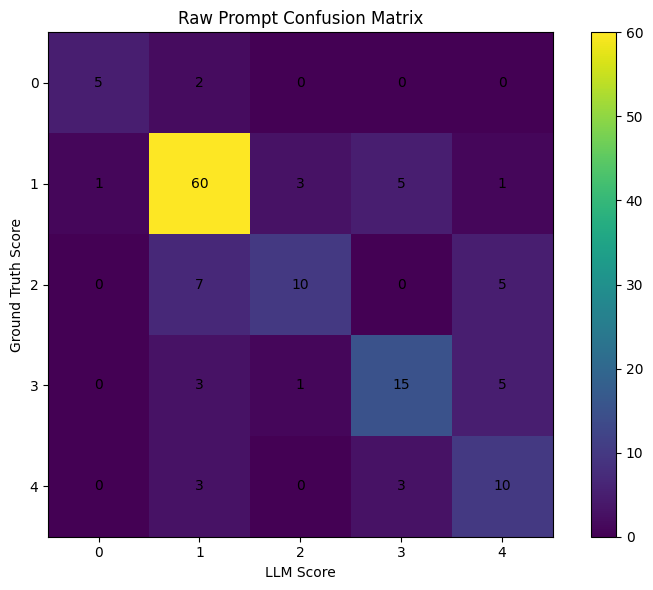
\includegraphics[width=\linewidth]{figures/raw_confusion_matrix.png}
\caption{Confusion Matrix for the Raw Prompt configuration.}
\label{fig:raw_matrix}
\end{figure}

Figure~\ref{fig:raw_matrix} illustrates the confusion matrix obtained using
the Raw Prompt strategy. The model correctly classified a large proportion
of reports assigned score 2 by human annotators. However, considerable
misclassification remained among the higher score categories, particularly
between scores 3, 4, and 5.

\begin{figure}[!t]
\centering
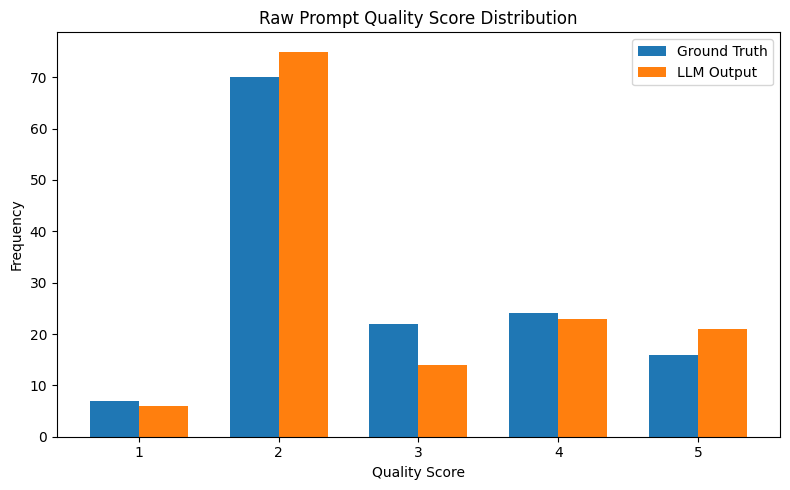
\includegraphics[width=\linewidth]{figures/raw_distribution.png}
\caption{Quality score distribution for the Raw Prompt configuration.}
\label{fig:raw_distribution}
\end{figure}

The score distribution shown in Figure~\ref{fig:raw_distribution}
demonstrates noticeable differences between the LLM-generated scores and
the human annotations. While the overall trend is similar, the Raw Prompt
configuration tends to overestimate some quality levels and underestimate
others, resulting in reduced agreement with the ground truth.

\subsection{Improved Prompt Results}

After refining the prompt design and introducing clearer evaluation
instructions, the model achieved improved performance across most metrics.

\begin{table}[!t]
\centering
\caption{Performance Metrics for Improved Prompt}
\label{tab:improved_results}
\begin{tabular}{lc}
\toprule
Metric & Value \\
\midrule
Accuracy & 76.26\% \\
Precision (Macro) & 57.09\% \\
Recall (Macro) & 55.58\% \\
F1-score (Macro) & 55.73\% \\
Cohen's Kappa & 0.3345 \\
\bottomrule
\end{tabular}
\end{table}

The Improved Prompt configuration achieved the highest overall Accuracy
(76.26\%) and Macro F1-score (55.73\%). These results indicate that prompt
engineering can positively influence the model's ability to assess bug
report quality.

\begin{figure}[!t]
\centering
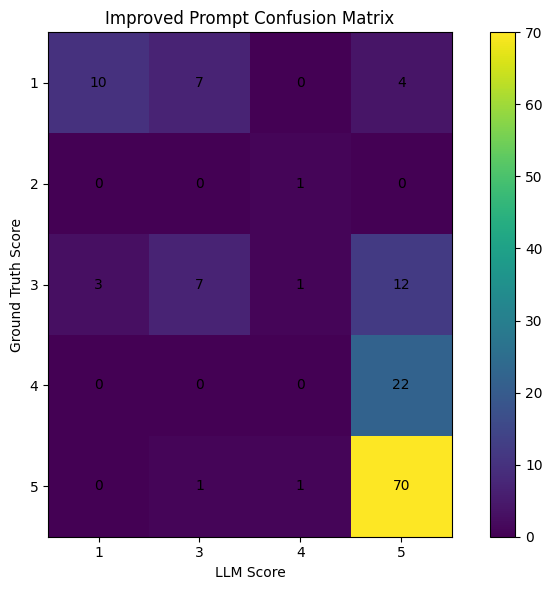
\includegraphics[width=\linewidth]{figures/improved_confusion_matrix.png}
\caption{Confusion Matrix for the Improved Prompt configuration.}
\label{fig:improved_matrix}
\end{figure}

Figure~\ref{fig:improved_matrix} shows that the Improved Prompt increased
the number of correctly predicted reports receiving the highest quality
score. Most reports rated highly by human annotators were also assigned
high scores by the LLM.

\begin{figure}[!t]
\centering
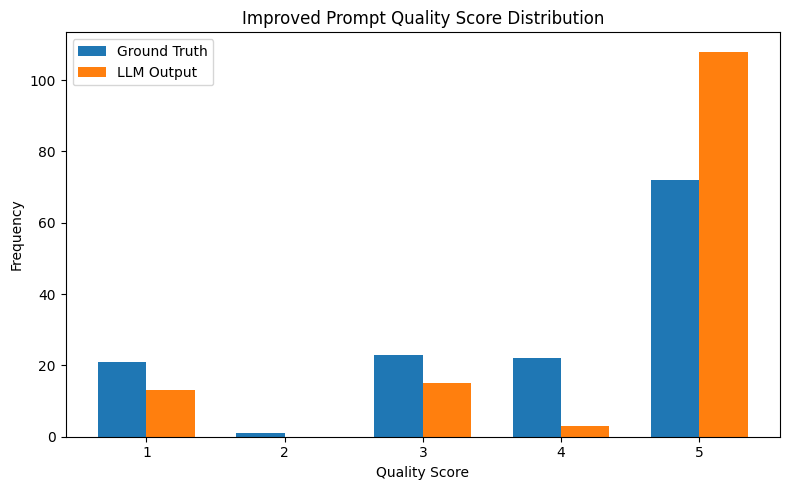
\includegraphics[width=\linewidth]{figures/improved_distribution.png}
\caption{Quality score distribution for the Improved Prompt configuration.}
\label{fig:improved_distribution}
\end{figure}

The distribution presented in Figure~\ref{fig:improved_distribution}
reveals a stronger concentration of predictions in the highest quality
category. Compared with the Raw Prompt, the Improved Prompt generated
outputs that more closely followed the overall pattern of the human
annotations.

\subsection{Comparison Between Prompt Configurations}

Table~\ref{tab:comparison} compares the performance of the two prompting
strategies.

\begin{table}[!t]
\centering
\caption{Comparison Between Raw and Improved Prompts}
\label{tab:comparison}
\begin{tabular}{lcc}
\toprule
Metric & Raw Prompt & Improved Prompt \\
\midrule
Accuracy & 69.18\% & 76.26\% \\
Precision (Macro) & 56.07\% & 57.09\% \\
Recall (Macro) & 55.01\% & 55.58\% \\
F1-score (Macro) & 53.22\% & 55.73\% \\
Cohen's Kappa & 0.5776 & 0.3345 \\
\bottomrule
\end{tabular}
\end{table}

The Improved Prompt outperformed the Raw Prompt on Accuracy, Precision,
Recall, and F1-score. Accuracy increased by approximately seven percentage
points, while the Macro F1-score improved from 53.22\% to 55.73\%.

Interestingly, Cohen's Kappa decreased from 0.5776 to 0.3345. This result
suggests that although the Improved Prompt produced more accurate
predictions overall, the score distribution became more concentrated in
certain categories, reducing agreement after correcting for chance.

\subsection{Distribution Analysis}

The confusion matrices and score distributions provide additional insight
into the behavior of the LLM. The Raw Prompt exhibited broader score
dispersion and more frequent confusion among neighboring categories. In
contrast, the Improved Prompt generated more consistent high-quality
predictions and reduced classification noise.

The distribution figures further indicate that prompt refinement helped the
model better recognize high-quality bug reports. However, the tendency to
assign high scores more frequently may also explain the reduction observed
in Cohen's Kappa.

\subsection{Summary of Findings}

The experimental results demonstrate that prompt engineering can improve
the performance of LLM-based bug report quality assessment. The Improved
Prompt achieved the highest Accuracy (76.26\%) and Macro F1-score
(55.73\%), indicating stronger alignment with human annotations.

Overall, the findings suggest that carefully designed prompts can enhance
the reliability of automated bug report evaluation, while also highlighting
the importance of considering both predictive performance and agreement
metrics when assessing LLM behavior.
\section{Discussion}
\label{sec:discussion}

\subsection{The Threshold Is Missed on Both Forms, but for Different Reasons}
\label{subsec:disc-finding}

Read strictly, the answer to the research question is negative on both forms:
GPT-4o mini reaches $\kappa = 0.578$ on Raw and $\kappa = 0.335$ on Improved,
neither meeting the pre-registered bar of $\kappa \geq 0.70$. But the two
shortfalls have different characters. On Raw the gap is narrow and symmetric:
the model sits just below \emph{substantial} agreement and close to the
$\kappa_{\text{control}} = 0.674$ measured between the two human annotators, and
its errors do not lean in any direction. On Improved the gap is wide and
one-sided: agreement is only \emph{fair}, far below the human ceiling on that
form ($0.556$), and driven by a significant optimistic bias. The Raw result is
consistent with a capable-but-imperfect evaluator; the Improved result is
consistent with an evaluator that is being misled.

\subsection{The Central Finding: Agreement Degrades on AI-Improved Reports}
\label{subsec:disc-gap}

The most important result of this study is the \emph{difference} between the two
forms. The same model, prompt, rubric, and scoring function, applied to the same
139 issues, agrees with humans far less well once those issues have been
rewritten by another LLM. The degradation is concentrated exactly where one
would expect if the model were responding to surface fluency rather than
substance: it is small on Steps to Reproduce (a checkable, structural judgment
that survives rewriting) and severe on Observed and Expected Behavior (free-text
sufficiency judgments that the ImproBR rewrite makes read as complete). The
bias test confirms the direction: on Improved the model scores higher than the
human in 47 of 52 disagreements and calls 111 of 139 reports reproducible. In
effect, the AI polish that makes a report look thorough also makes the evaluator
credit it, whether or not the underlying reproducibility information is really
there.

This has a concrete practical implication. Modern triage pipelines increasingly
contain LLM-generated or LLM-rewritten text, and a natural design is to chain an
LLM improver with an LLM evaluator. Our results warn that such a chain can be
self-reinforcing: the evaluator systematically over-credits the improver's
output. An LLM evaluator should therefore be validated on the specific kind of
text it will score in deployment---validating it only on raw human reports would
have overstated its reliability on the improved reports by nearly $0.25$ kappa.

\subsection{Agreement Is Uneven Across Dimensions, Consistently}
\label{subsec:disc-dimensions}

On both forms the dimension ranking is identical: Steps to Reproduce is
strongest (Raw $\kappa = 0.693$, Improved $0.654$), Expected Behavior is
intermediate, and Observed Behavior is weakest (Raw $0.289$, Improved $0.130$).
Steps to Reproduce is closest to a binary, checkable judgment---does the report
state enough to attempt the action---while Observed Behavior sufficiency
requires judging whether a free-text description is complete enough, a more
subjective distinction. That the same ordering holds on both forms, while the
softer dimensions degrade much more under rewriting, suggests an LLM-as-evaluator
is more trustworthy for structurally checkable sub-judgments than for open-ended
sufficiency judgments, and that this is a stable property of the model rather
than an artifact of one dataset.

\subsection{Coarse Screening Survives on Both Forms}
\label{subsec:disc-binarized}

The binarized check (score $\geq 4$ as reproducible) reaches $87.1\%$ accuracy
on Raw and $86.3\%$ on Improved, in both cases noticeably stronger than the
fine-grained ordinal agreement. Most of the model's disagreement with humans
happens between adjacent ordinal categories rather than between clearly
reproducible and clearly not. Practically, GPT-4o mini is more dependable as a
coarse first-pass filter than as a fine-grained 1--5 scorer---though on the
Improved form the high binary recall ($98.9\%$) comes at the cost of precision,
because the model calls almost everything reproducible, so even the coarse
filter inherits the optimistic bias when the input has been AI-polished.

\subsection{Relation to Prior Work}
\label{subsec:disc-related}

ImproBR reports that its pipeline raises the share of Executable reports from
$28.8\%$ to $67.6\%$ on this dataset~\cite{akyol2026improbr}; our human
ground truth reproduces those exact figures, confirming that we are evaluating
on the same material. Our contribution is complementary and cautionary: rather
than improving reports, we ask whether an LLM can \emph{judge} their
reproducibility with human-level reliability, and we find that it approaches
that bar on original reports but falls well short on the very reports ImproBR
improves. Combined with the LLM-as-judge literature's caution that automated
evaluators must be validated against human labels before their agreement figures
can be trusted~\cite{li2024judges}, our result sharpens that caution: validation
must be done on the same distribution of text---including AI-generated
text---that the evaluator will face in use, because agreement measured on human
reports does not transfer to machine-rewritten ones.

\section{Threats to Validity}
\label{sec:threats}

\subsection{Internal Validity}
 
The primary threat is \emph{model non-determinism between runs or versions}. We mitigate this by using a fixed model snapshot (\texttt{gpt-4o-mini-2024-07-18} rather than a model alias), setting temperature to 0 for deterministic generation, and locking the prompt template to a single version throughout all 139 reports.
 
Another threat is \emph{prompt design bias}, where the wording could inadvertently shift the LLM's scoring behavior. We reduce this through a clearly defined ordinal rubric (scale 1--5), and we use a controlled fallback strategy (zero-shot $\to$ few-shot only under predefined pilot conditions) rather than iterative prompt refinement.
 
\subsection{Construct Validity}
 
A key concern is whether we are truly measuring ``reproducibility.'' Potential threats include misalignment between how humans and LLMs interpret reproducibility, and dependence on structured extraction (Steps to Reproduce, Expected/Observed Behavior) that may introduce abstraction bias.
 
We address this by anchoring the LLM rubric to the existing human annotation guidelines in the dataset, using the same ordinal scale for both human and LLM evaluation, and analyzing agreement separately for each reproducibility dimension (Steps, Observed Behavior, Expected Behavior) to reduce over-abstraction from a single composite score.
 
\subsection{External Validity}
 
The study is limited to Mojira Minecraft bug reports, an open-source game development context. Results may not generalize to enterprise bug tracking systems or other domains with different reporting standards.
 
However, the dataset spans diverse technical bug types and is directly comparable to prior OSS studies. The measurement protocol itself is domain-agnostic and can be replicated on other issue trackers.
 
\subsection{Conclusion Validity}
 
Cohen's Kappa can be sensitive to class imbalance in ordinal scores, and bootstrap confidence intervals may fluctuate depending on resampling variance. The Wilcoxon signed-rank test assumes symmetric pair-wise differences.
 
We mitigate these by computing bootstrap confidence intervals for $\kappa$ rather than relying on asymptotic assumptions, using non-parametric Wilcoxon testing (appropriate for ordinal data), and reporting effect sizes (rank-biserial correlation) alongside $p$-values.
 
\subsection{Reproducibility}
 
To ensure our results are reproducible, we fix the dataset to 139 Mojira reports, pin the model version explicitly, lock the prompt template, remove randomness from sampling, and use standard statistical libraries (scikit-learn, scipy).
 
\section{Conclusion}
\label{sec:conclusion}
This study measures the degree to which an LLM-based reproducibility evaluator aligns with developer manual review on bug reports from Mojira Minecraft. Using GPT-4o mini and 139 pre-annotated reports, we assess agreement through Cohen's Kappa, targeting a threshold of $\kappa \geq 0.70$ as evidence of substantial agreement.
 
Our findings have direct implications for software maintenance: if LLMs can achieve this level of alignment, they become a viable first-pass filter in bug triage workflows, reducing manual review burden.
 
Beyond this dataset, the measurement protocol we establish---comparing LLM evaluation to human judgment using Cohen's Kappa---can be adapted to any OSS project seeking empirical validation before deploying LLM-based issue filtering. This creates a reusable benchmark for the broader community.
 
Future work should extend this evaluation across multiple repositories and issue trackers (GitHub, GitLab) to assess generalization, explore human-in-the-loop workflows where LLM scores trigger developer review rather than replacing it, and investigate fine-tuning or few-shot prompting to improve alignment on report sections that cause systematic disagreement.
 

\bibliographystyle{IEEEtran}
\bibliography{references}

\end{document}

% bảng đẹp hơn